\documentclass[conference]{IEEEtran}
\IEEEoverridecommandlockouts
% The preceding line is only needed to identify funding in the first footnote. If that is unneeded, please comment it out.
\usepackage{cite}
\usepackage{amsmath,amssymb,amsfonts}
\usepackage{algorithmic}
\usepackage{graphicx}
\usepackage{textcomp}
\usepackage{xcolor}
\usepackage{verbatim}
\usepackage{subfigure}
\def\BibTeX{{\rm B\kern-.05em{\sc i\kern-.025em b}\kern-.08em
    T\kern-.1667em\lower.7ex\hbox{E}\kern-.125emX}}

%% Bibliography1

\begin{document}

\title{Attack-Defense Trees}

\author{\IEEEauthorblockN{Benjamin \c Coban}
\IEEEauthorblockA{\textit{Eberhard Karls University Tübingen} \\
\textit{Embedded Systems}\\
Tübingen, D \\
Benjamin.Coban@student.uni-tuebingen.de}
}

\maketitle

\section*{Content}
The ability to investigate an attack scenario for a given security system enforces a formal model in order to describe and evaluate security measurements. The \textit{Attack Defense Trees (ADTrees)} serve as a tool to describe and evaluate an attack defense scenario using attributes. \\
This report addresses the paper \textit{Attack-Defense Trees} written by the \textit{Security and Trust of Software Systems} Department of the University of Luxembourg, \texttt{SaToSS} in short, published in 2014. \cite{dblp} Furthermore, this report is based on the already held presentation to this topic during this very seminar.
\\\\
\begin{IEEEkeywords}
Attack Trees, ADTerms, Attribute Domains
\end{IEEEkeywords}
\section{Introduction}
%Security bla
It is widely known that the security of a system seen as property is not static. Therefore, there cannot exist a general algorithm deciding whether or not a given system is secure in its sense. IT-Security Architects and Engineers are stuck with persistent research of bug reports of the technology the respective enterprise is using. In the industry, IT security is one use case of many others. The types of systems to examine vary depending on context. For instance, the construction of a museum is considered as a system and it is of interest to guarantee that the objects, stored in this kind of facility, are considered safe and sound. In consequence, it is urgent to establish a formal model for system description and security evaluation. There are various challenges to overcome, for instance:
\begin{itemize}
	\item What are the best defensive measures to invest in?
	\item How can it be decided whether a defensive measure from the past is still necessary?
	\item How can newly discovered attacks be efficiently documented?
\end{itemize}
%
%	Attack Tree kurz 
%
The so-called \textit{Attack Trees} were a first approach to formalize a model in order to evaluate the security of complex systems. They are a tree-like representation of an attack scenario and one is able to identify weaknesses in security systems. However, this model exhibits several limitations. The interactions between attackers and defenders are not captured in any way, making a precise defense analysis impossible. In order to overcome this limitations, the model needed to be extended for a higher granularity in an attack defense scenario.\\
The \textit{Attack Defense Trees} - ADTrees in short - fulfill these necessities. ADTrees portray an attack defense scenario as a game between a proponent and opponent. In order to further analyze ADTrees, syntax and semantics have to be defined. Only then will approaches for quantitative analysis formally work.


\section{Terminology}
%%Graphentheorie
A \textit{graph} $G=(V,E)$ is a tuple consisting of two sets - the set of vertices and the set of edges. An \textit{edge} $e = (v,w), v,w \in V$ is a tuple and describes a connectivity relation between two vertices. Unless otherwise mentioned, the graphs are \textit{undirected}, meaning that the edge $(u,v)$ is identical to the edge $(v,u)$,$u,v\in V$. A \textit{Tree} $T$ is a connected acyclic undirected graph. 
% Tree
A tree is \textit{rooted} iff there exists one vertex labelled as \textit{root}.\cite[p.42]{GD} A \textit{leaf} is a node with degree 1. An \textit{inner node} is a node of a tree which is not a root and not a leaf. Leaves and inner nodes must have one parent. \cite[p.34]{Cormen} A cycle in a graph is a finite path, with the same node at start and the end. A directed acyclic graph (in short DAG) is a directed graph that does not include any cycles.
\section{Attack Defense Trees (ADTrees)}
An \textit{ADTree} is a node-labelled rooted tree describing the measures of an attacker and the respective countermeasures of the defender as a game scenario where the proponents goal is represented by the root of the ADTree. The vertices of an ADTree are labelled either as \textit{attacker} or \textit{defender}, representing sub-goals of the pro- or opponent. There are two features in the ADTree - a \textit{refinement} is sub-dividing a goal into their sub-goals, whereas a \textit{countermeasure} illustrates a conflict scenario between the proponent and the opponent. A refinement is either \textit{conjunctive} or \textit{disjunctive}, meaning that in order to achieve a parent goal, either \textit{all} of the subgoal or \textit{at least one} subgoal have to be satisfied. Non-refined nodes represent \textit{basic actions}.\\
When illustrating ADTrees, defensive labelled nodes will be drawn in rectangles and offensive labelled nodes will be drawn in circles. The refinements as described above will be connected with a circular arc to illustrate a conjunction. In the following example, the reader can comprehend the general idea of ADTrees and the two types of refinements.
%Example
\subsection{A small example}
Since ADTrees are described as labelled graphs, it is quite easy to get an idea of the functionality and interpretation by considering the drawing of an example graph. Figure \ref{theft} illustrates a facility where jewelry is stored. A thief - the proponent of the scenario as game - tries to overcome several hurdles in order to steal the jewelry. The thief needs to overpower security guards and destroy shatterproof glass for the theft. The goal lies in the root.
\begin{figure}[htbp]
	\centering
		\centerline{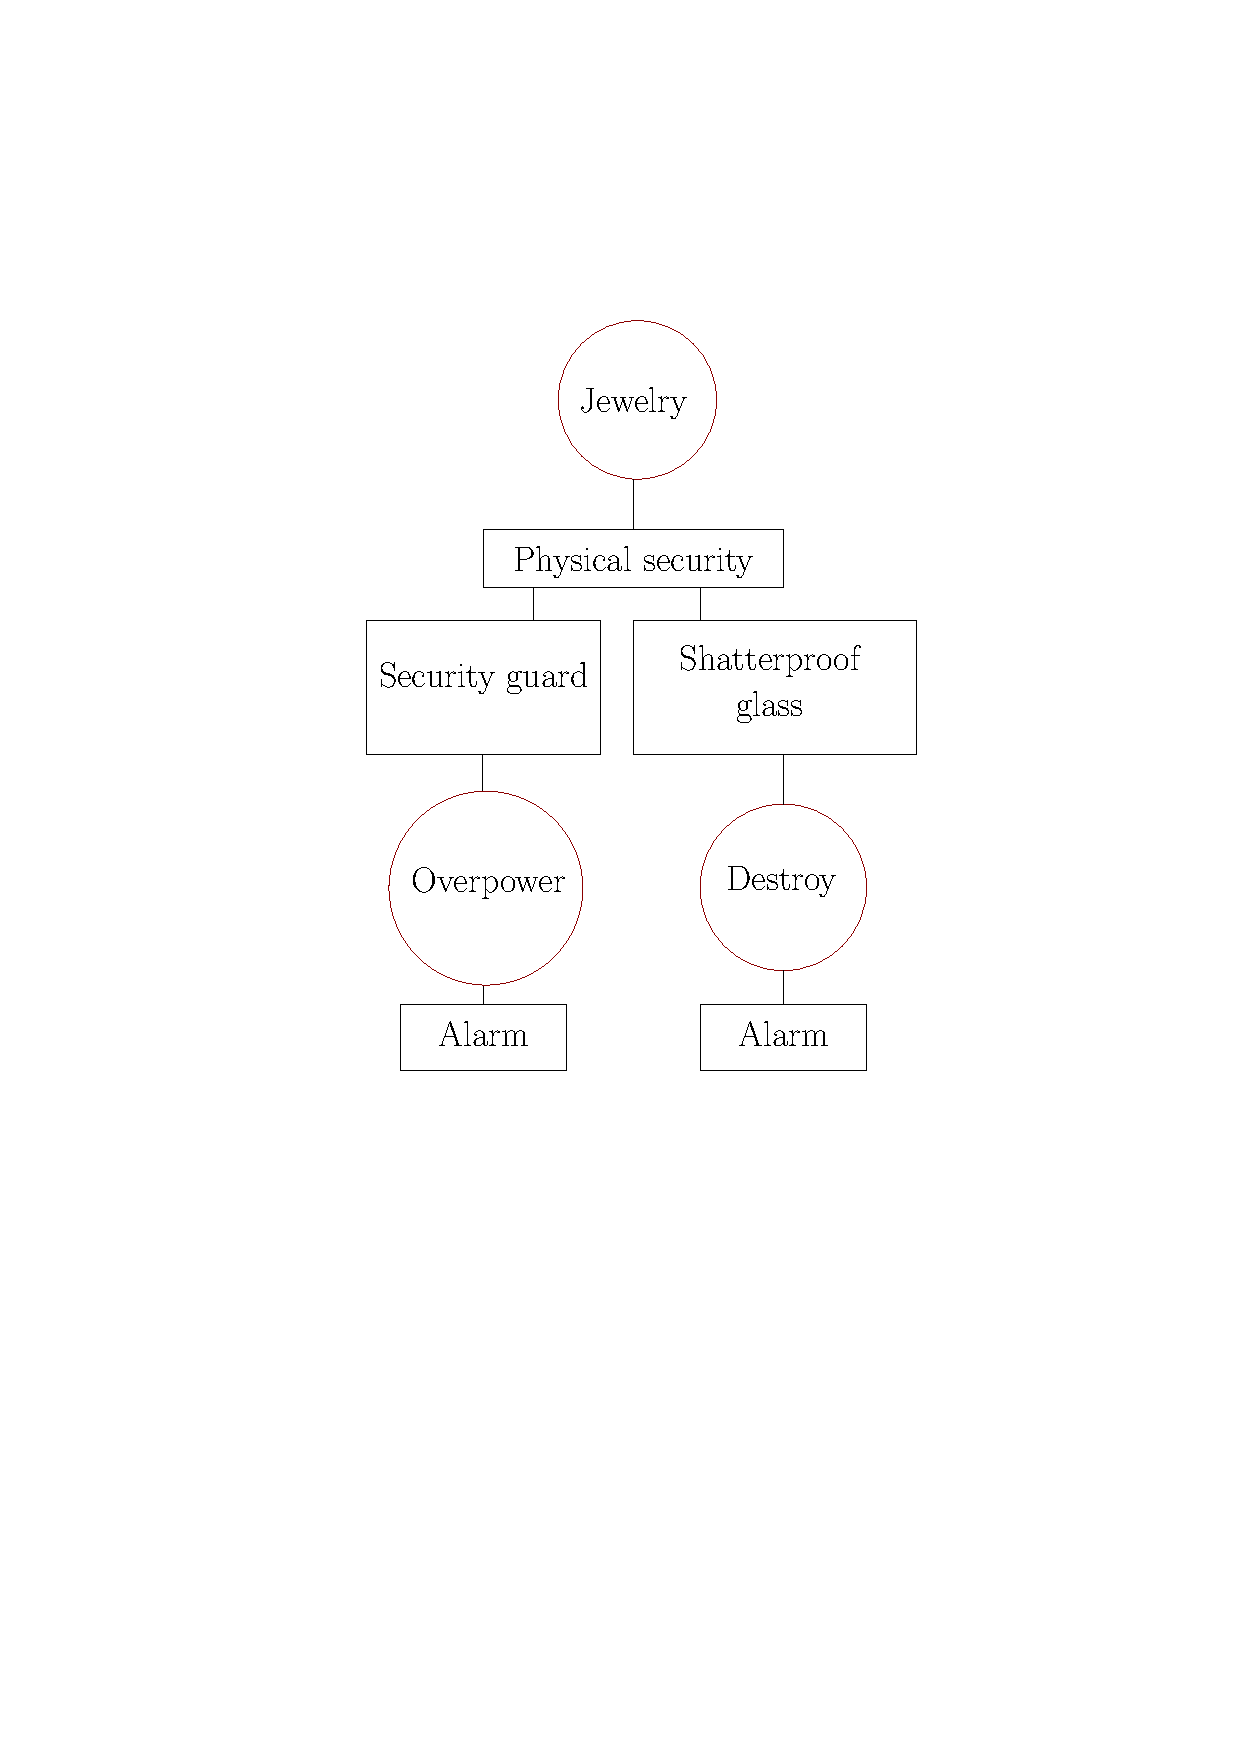
\includegraphics[width=0.5\linewidth,page=1]{graphics.pdf}}
		\caption{An AD(Sub-)Tree for a thief trying to steal jewelry}
		\label{theft}
\end{figure}
In figure \ref{ref}, refinements for a thief to defeat a guard are illustrated. The disjunction lies in the children \texttt{Steal Keys}, \texttt{Overpower} and \texttt{Bribe}. At least one of those subgoals has to be achieved to defeat the guard. If an attacker would choose overpowering, the conjunction of its children indicate that the attack must have more guys with guns during the attack. Both subgoals must be achieved.
\begin{figure}[htbp]
	\centering
	\centerline{\includegraphics[width=0.85\linewidth,page=2]{graphics.pdf}}
	\caption{An AD(Sub-)Tree for a thief trying to defeat a guard - there are multiple options}
	\label{ref}
\end{figure}
%
\\\\
Now, the definition of ADTrees delivers a model for scenario representation. But there is still much more left to focus on, a graph model is not sufficient for evaluating semantics from a theoretical point of view. By now, we lack in tools when we want to investigate whether or not two given ADTrees are formally equivalent. We do not even know, what equivalency means in context of ADTrees. So, the next step will introduce \textit{syntax} for ADTrees in order to enable an approach to denote ADTrees in an already known scheme - in terms. These terms will be fundamental for introducing propositional semantics.
\section{Abstract syntax: ADTerms}
As widely known, terms need some sort of alphabet to be defined on just like any word of any language. An \textit{AD-signature} $\Sigma = (S,F)$ is a tuple consisting of a a set of types $S$ and a set of function symbols $F$, where:
\begin{itemize}
	\item $S = \{p,o\}$ label proponent or opponent objects, respectively
	\item $F$ is a union of typed constants $\mathbb{B}$, conjunctive or disjunctive refinements $(\vee,\wedge)$ and a binary function $c$ to connect countermeasures from a player to its opposing player. Let $s \in S$.
	$$F = \mathbb{B}^s \cup \{\vee^s,\wedge^s\}\cup c^s$$
\end{itemize}
An \textit{ADTerm} $t$ is a finite typed ground term over an AD-signature $\Sigma$. \\
In the next subsection, we will see the correspondance between ADTrees and ADTerms. So far, an ADTree is defined as an extension of the Attack Tree model, therefore a labelled tree. With help of ADTerms and AD-signatures, there will be a new definition of ADTrees.
\subsection{ADTrees $\Leftrightarrow$ ADTerms}
With help of an ordering of the nodes of a tree, a \textit{finite ordered tree over a set of labels} is a \underline{function} where each node of the tree with its number is identified with a label. The ordering of the tree corresponds to the location in the tree. Starting from the root, the ordering will traverse according to a BFS of the graph. The resulting drawing will place the children from left to right and from top to bottom. Then, the following defintion holds:\\
An ADTree is a finite ordered tree $T$ over the set of labels $L_T = \mathbb{B}^p \cup \mathbb{B}^o \{\vee^p,\vee^o,\wedge^p,\wedge^o\}$. The index will be used as declaration of relation the following way: Let $v_1,v_2 \in V_T$. Then, if \texttt{index}$(v_1)$ is a multiple of \texttt{index}$(v_2)$, then there is a refinement. This stops at a typed constant, since the trees are finite. If \texttt{index}$(v_2)$ and \texttt{index}$(v_1)$ do not share a common divisor, then they differ in their label. Crucial is the root of the tree, since it determines the proponent. Moreover, each node has at most one child of the opposite type.\\
With this definition, it is now possible to obtain an ADTerm $t_T$ for a given ADTree $T$. 
\subsection{The refinement example tree as ADTerm}
Recall Figure \ref{ref}. The corresponding ADTerm is denoted as:
\begin{align*}
\small
	c^o\left(\text{SecGuard}, c^p \left( \vee^p \left( \text{StealKeys}, \wedge^p \left( \text{Outnum},\text{Weapons} \right), \text{Bribe}  \right)  \right) \right)
\end{align*}
Note, that the \texttt{Overpower }node is substituted with the conjunction of its children. 
\section{Design choices of this model}
When creating a model, one could have to overcome several difficulties - it is beneficial to keep the \textit{usability} in mind, since attack defense scenarioes vary strongly in different use cases. Another aspect is the \textit{complexity }of this model. Complex systems have to be illustrated adequately with the least possible complexity overhead. Still, the functionality of the model must not suffer by induced restrictions. It is a thin line of creating a model with a high complexity in one hand and losing functionality on the other hand.\\Hence, the authors of this paper concluded several design choices, which ensure a useful, handy tool derivation with strong functionalities.\\
Refinements are restricted to one type only per node - a node may have either a conjunctive or a disjunctive refinement. If there was the necessity of both refinements, then this hurdle is overcome by creating a subnode with the respective other refinement. Furthermore, a node may have at most one child of opposite type. This restrictions for children do not limit the expressiveness of the formalism. The reader might recall that every propositional formula can be equivalentally converted to a formula which is a finite conjunction or disjunction of subformulas.\\
For the sake of simplicity, the authors restricted the extension to finite trees and \textit{excluded} DAGs in terms of model extension. It is common practice to extend an existing model in baby steps. Without infinite trees, not all recursive defined scenarioes can be modelled. Therefore, the evolution of a defense system exposed to automated attacks is bounded.
\section{Propositional semantics}
With ADTerms based on AD-signatures, it is now possible to introduce \textit{semantics} on this \textit{syntax}. In this section, propositional semantics for ADTerms will be defined since it is the most frequently used semantics for Attack Trees. Then, the satisfiability of the formula represented by an ADTerm will model the feasibility of the scenario illustrated by this very term.\\
A semantics for ADTerms is an type-preserving equivalence relation on the set of all ADTerms. For instance, the term $t_1 = \texttt{Overpower} \vee \texttt{Overpower}$ shall be element of the very equivalency class represented by $t = \texttt{Overpower}$. The steps necessary to evaluate an ADTerm with propositional logic is quite easy and are defined inductively.
\begin{itemize}
	\item Substitute every basic action of the term with a propositional variable. Conjunctive and disjunctive refinements in an ADTree will correspond to conjunctions and disjunctions of the subtrees as formulas. 
	\item Countermeasures will be transferred the following way:
	$$c^p(t_1,t_2)\Leftrightarrow t_1 \wedge \neg t_2~~~~~~ p \in P $$
	This means that the proponent must hold its subgoal $t_1$ whereas the opponent must fail with its subgoal $t_2$.
\end{itemize}
As seen, it is pretty convenient to interpret a given ADTerm as a propositional formula. With this information, one is able to implement a framework for ADTrees with semantics in any given programming language. The authors provide a first implementation, called \text{ADtool2}, which will be discussed in the summary.
\subsection{The example as a propositional formula}
Recall Figure \ref{ref} again with its ADTerm.
\begin{align*}
\small
c^o\left(\text{SecGuard}, c^p \left( \vee^p \left( \text{StealKeys}, \wedge^p \left( \text{Outnum},\text{Weapons} \right), \text{Bribe}  \right)  \right) \right)
\end{align*}
It is fairly easy to comprehend the following derived propositional formula:
\begin{align*}
\text{StealKeys} \vee \left( \text{Outnumber}\wedge\text{Weapons} \right) \vee \text{Bribe}
\end{align*}
\section{Attributes}
With syntax and semantics, all left to implement is a way of describing algorithms based on given scenarioes and points of interest to evaluate. \textit{Attributes} will serve as an approach to quantitatively evaluate given scenarioes and attacks. As a syntax needs an alphabet, an attribute needs a \textit{domain} to work on. An attribute domain works like some kind of mapping for a given ADTerm with its typed constants.\\
An \textit{Attribute Domain} $A_\alpha$ is a tuple, consisting of a set of values $D$ and functions defined on that set of values.
$$A_\alpha = \{D,\vee^o_D,\vee^p_D,\wedge^o_D,\wedge^p_D\}$$
One result of this approach is that every ADTerm will be evaluable for any given consistent attribute domain.
\subsection{An example for an attribute domain}
Consider the following domain:
\begin{align}
A_\text{sat} &= \{ \{0,1\},\vee,\wedge,\vee,\wedge, \star, \star\}\\
x \star y &:= x \wedge \neg y
\end{align}
Then, $A_\text{sat}$ will be the attribute domain to evaluate the satisfiability of the proponents goal modelled by the root.\\\\
The evaluation of an ADTerm will work \textit{bottom-up}, meaning, that the leaf nodes will be substituted with a value out of the set of values given by $A_\alpha$ and afterwards, with help of the refinement / countermeasure mapping of $A_\alpha$, the evaluation takes place up to the root. This way of evaluation is a rather simple, yet effective one in terms of complexity, implementation and general understanding.
\subsection{Exemplary calculation of minimal costs}
In the following example, the way to implement a minimal cost function is illustrated. Consider the following attribute and its domain for Figure \ref{ref}:
\begin{align*}
	A_{\text{cost}} = \left(\mathbb{R}^+\cup\{\infty\},\min,\cdot,+,\min,+\min\right)
\end{align*}
The conjunctions and disjunction refinements and countermeasures are set to binary functions - the minimum function, simple addition and multiplication. Furthermore, a cost function $\beta$ is introduced:
\begin{align*}
\beta(\text{Weapons}) &= 500\\
\beta(Outnum) &= 4\\
\beta(\text{Keys}) &= \infty\\
\beta(\text{Bribe}) &= 10000
\end{align*}
In a scenario where it is impossible to obtain the master key, the cost function is set to infinity. The term $t$ holds as followed:
\begin{align*}
t = \vee^p \left( \text{StealKeys}, \wedge^p \left( \text{Outnum},\text{Weapons} \right), \text{Bribe}  \right)
\end{align*}
And the minimal costs would be calculated the following way:
\begin{quotation}
	$\Rightarrow$ cost$(t)= \left( \min \left( \infty, \cdot \left( 4,500\right), 10000 \right)  \right) = 2000$
\end{quotation}
Now, with backtracking, the user is possible to identify the assignment in the corresponding propositional formula and will attack with a lot of guys with lots of weapons.
\section{Summary}
%% ADTrees represent a security system evolution
With ADTrees, a graph representation of complex systems was established. In order to implement graph algorithms, the equivalency of ADTrees to ADTerms derived from propositional logics was necessary to establish. 
%% deliver a language to operate on
Therefore, every ADTree is respresented by an ADTerm and every ADTerm can be drawn as a tree. With the propositional logic induced by ADTerms, the fundamental work for quantitative algorithms has been done. 
%% Attributes deliver a base to evaluate a given system
Attributes can be used to analyze specific problems and based on the situation, a certain attribute domain is picked. 
\\
One of the greatest strengths of this model is the simplicity of application in a high variety of fields of work. Whenever there is something to protect, then there exists a suiting scenario describing the circumstances, consequences and potential threats. This model is also suitable for penetration testing - the root of the corresponding ADTree is then just to find a bug in a software, an unsecure cipher in usage or infrastructural flaws.\\
On $\text{Github}^\copyright$\cite{github}, the SaToSS uploaded a first implementation of an ADTree framework called \textit{ADTool2}, written in Java and built with Maven. There, the reader may find example outputs of given scenarioes.\\
With a little working in the framework, the user gets a satisfying amount of functionalities - basic operations like creating, altering, saving and deleting ADTrees. Defining and applying own attributes for specific use cases are included. It seems like this tool might just suit for basic applications.
\section{Future Work}
As already mentioned, one  of the most obvious limitations of the model is the missing dependency formalism between two arbitrary nodes. In order to overcome this gap the model should be extended to a subclass of \textit{(DAGs)}. With DAGs, dependencies and execution order of goals may be introduced and evaluated. One other point of interest are infinite trees in order to document system behaviour for e.g. automated attacks adequately.
\begin{thebibliography}{00}
\bibitem{Cormen} T. Cormen, C. Leiserson, R. Rivest, and C. Stein, ``Introduction To Algorithms, 3rd Edition,'', 2009
\bibitem{GD} G. Di Battista, P. Eades, R. Tamassia, I. Tollis, ``Graph Drawing: Algorithms for the Visualization of Graphs,'', 1999
\bibitem{dblp} https://dblp.org/pers/k/Kordy:Barbara.html, visited 27.3.2020
\bibitem{github} https://github.com/tahti/ADTool2, visited 29.3.2020
\end{thebibliography}
\end{document}
